\section{Zusammenfassung und Ausblick}\label{sec:02_05_zusammenfassung}

Dieser Abschnitt beschäftigt sich mit ein paar Eckdaten zur EU und versucht die in einige Zahlen zusammenzufassen (siehe Abb~\ref{fig:euroEckDaten}).
\noindent
\begin{figure}[H]
\centering
    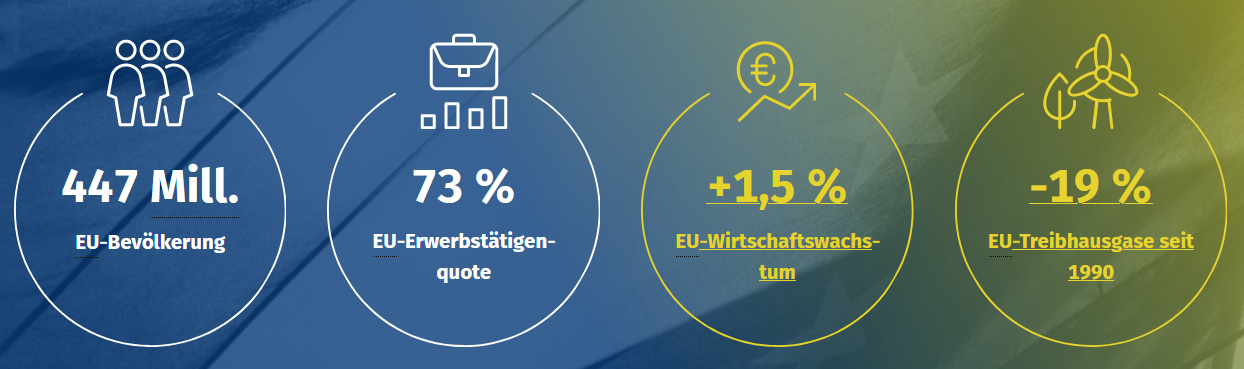
\includegraphics[width=.6\textwidth]{images/EU_Eckdaten.PNG}
    \caption{Die Eckdaten der EU}
    \textbf{Quelle: }  \cite{euroInZahlen}
    \label{fig:euroEckDaten}
\end{figure}

\subsection{Die Bevölkerung}\label{subsec:EuroBevoelkerung}

Die EU umfasst 447 Millionen Einwohner auf den 27 Länder verteilt:
\noindent
\newcolumntype{s}{>{\columncolor{EUBlue}} m{2.5em}}
\newcolumntype{g}{>{\columncolor{Gray}} m{4em}}
\begin{table}[ht]
\caption{Die EU Bevölkerung}
\label{tab:euBevoelkerung}
\centering
\begin{tabular}{s|g|g|g|g|g|g}
\hline
Staat &Belgien &Deutsch- land &Frank- reich &Italien &Luxem- burg &Nieder- lande \\
\hline
2019~\tablefootnote{In Millionen} &11,5 &83,0 &67,0 &60,4 &0,6 &17,3 \\
\hline
2060~\tablefootnote{Eurostat-Bevölkerungsvorausberechnung basierend auf 2019} &11,9 &81,8 &69,7 &56,0 &0,8 &18,0 \\
\hline
\hline
Staat &Dänemark &Irland &Griechen- land &Portugal &Spanien &Finnland \\
\hline
2019 &5,8 &4,9 &10,7 &10,3 &46,9 &5,5 \\
\hline
2060 &6,1 &6,4 &9,0 &8,9 &48,4 &5,2 \\
\hline
\hline
Staat &Öster- reich &Schweden &Estland &Lettland &Litauen &Malta \\
\hline
2019 &8,9 &10,2 &1,3 &1,9 &2,8 &0,5 \\
\hline
2060 &9,3 &12,7 &1,2 &1,3 &2,0 &0,7 \\
\hline
\hline
Staat &Polen &Slowakei &Slowenien &Tschechien &Ungarn &Zypern\\
\hline
2019 &38,0 &5,5 &2,1 &10,6 &9,8 &0,9 \\
\hline
2060 &32,5 &5,0 &2,0 &10,4 &9,1 &1,1 \\
\hline
\hline
Staat &Bulgarien &Rumänien &Kroatien &Die EU &Vereinigtes Königreich &Die EU mit UK\\
\hline
2019 &7,0 &19,4 &4,1 &446,8 &66,6 &513,4 \\
\hline
2060 &5,3 &14,5 &3,2 &432,5 &- &- \\
\hline
\end{tabular}
\end{table}
\newpage

\subsection{Der Arbeitsmarkt}\label{subsec:EuroArbeitsmarkt}

Die Erwerbstätigenquote in der EU liegt bei 73\% und die Erwerbslosenquote bei 6,6\%.
\noindent
\newcolumntype{s}{>{\columncolor{EUBlue}} m{2.5em}}
\newcolumntype{g}{>{\columncolor{Gray}} m{4em}}
\begin{table}[ht]
\caption{Die EU-Erwerbstätigenquote und Erwerbslosenquote (20- bis 64-Jährige)}
\label{tab:euErwerbtaetigenquote}
\centering
\begin{tabular}{s|g|g|g|g|g|g}
\hline
Staat &Belgien &Deutsch- land &Frank- reich &Italien &Luxem- burg &Nieder- lande \\
\hline
ET~\tablefootnote{Erwerbstätigenquote} &70,5 &80,6 &71,6 &63,5 &72,8 &80,1 \\
\hline
EL~\tablefootnote{Erwerbslosenquote} &5,2 &3,1 &8,2 &9,9 &5,3 &3,0 \\
\hline
\hline
Staat &Dänemark &Irland &Griechenland &Portugal &Spanien &Finnland \\
\hline
ET &78,3 &75,1 &61,2 &76,1 &68,0 &77,2 \\
\hline
EL &4,7 &4,6 &17,3 &6,4 &13,8 &6,1 \\
\hline
\hline
Staat &Öster- reich &Schweden &Estland &Lettland &Litauen &Malta \\
\hline
ET &8,9 &10,2 &1,3 &1,9 &2,8 &0,5 \\
\hline
EL &9,3 &12,7 &1,2 &1,3 &2,0 &0,7 \\
\hline
\hline
Staat &Polen &Slowakei &Slowenien &Tschechien &Ungarn &Zypern\\
\hline
ET &73,0 &73,4 &76,4 &80,3 &75,3 &75,7 \\
\hline
EL &3,2 &5,6 &4,4 &2,0 &3,3 &7,0 \\
\hline
\hline
Staat &Bulgarien &Rumänien &Kroatien &Die EU &Vereinigtes Königreich &Die EU mit UK\\
\hline
ET &75,0 &70,9 &66,7 &73,1 &79,3 &- \\
\hline
EL &4,2 &3,7 &6,4 &6,6 &3,4 &- \\
\hline
\end{tabular}
\end{table}

\subsection{Die Wirtschaft}\label{subsec:EuroWirtschaft}

Das nominale Bruttoinlandsprodukt (BIP) der EU beträgt 13.923 Milliarden Euro und der Kaufkraftstandards (\gls{kks}) pro Einwohner liegt Europa weit bei 30.158 Euro. An der Spitze steht Deutschland mit 3.435 Milliarden Euro (BIP) und 37.050 Euro Kaufkraftstandards. Das Schlußlicht ist hier Malta was den BIP angeht mit 13 Milliarden Euro und Bulgarien mit 15.424 Euro was den Kaufkraftstandards anbelangt. 